%\documentclass{article}
\documentclass[conference,10pt,twocolumn]{./IEEE/IEEEtran}
\usepackage{tabularx}
\usepackage{ulem}
\usepackage{verbatim}
\usepackage{listings}
\usepackage{xcolor}
\usepackage{textcomp}
%\usepackage{graphicx}

 \ifCLASSINFOpdf
    \usepackage[pdftex]{graphicx}
    \graphicspath{{./}{../}}
    \DeclareGraphicsExtensions{.pdf,.jpeg,.png}
 \else
    \usepackage[dvips]{graphicx}
    \graphicspath{{../}}
  \DeclareGraphicsExtensions{.eps}
\fi

%\usepackage{colt11e}
%\usepackage{amsmath}
%\usepackage{amssymb}
%\usepackage{pseudocode}
%\usepackage{dsfont}
%\usepackage{url}

%\input{Macros}

\title{Java Program Execution Analysis Tool}

\author{
  Dongyang Zhang \\
  {\fontsize{10}{11}\selectfont University of Texas, Austin}\\ 
  \texttt{dyz@utexas.edu}
\and
  Jeremy Joachim \\
  {\fontsize{10}{11}\selectfont University of Texas, Austin}\\ 
  \texttt{jajoachim@gmail.com}
}

\begin{document}
\maketitle

\section{Abstract}
Automated instrumentation of compiled code is a valuable resource for programmers who wish to analyze their programs.
This paper presents one such tool called the Java Dyanmic Analyzer which is built upon the Javassist and JUNG libraries.
It comes with various instrumentation options to gather data which is displayed with an interactive GUI upon the instrumented program’s main function exit.

\section{Introduction}
It is well known that software testing and profiling is the majority component to software development.
This makes automated techniques extremely valuable to software developers.
Automated techniques often take the form of instrumentation because it can be loaded post-compilation and requires minimal intervention on the programmer’s side.
There are several instrumentation systems for Java coding, however they tend to have narrow purposes.
The most popular focuses are code coverage and performance evaluation.
In this paper, we provide a system that focuses on covering a breadth of subjects rather than the depth of a few. 
The Java Dynamic Analyzer (JDA) provides data on both performance evaluation and code coverage while remaining easily configurable.

\section{Previous Work}
There are two notable systems that the JDA competes with.
The first is called JVisualVM \cite{VisualVM}, which focuses on performance analysis.
It provides detailed information about method execution times via instrumentation, however the actual performance hit taken from the instrumentation is surprisingly small.
Additionally, The instrumentation is applied during a program’s execution rather than as a precursor.
JVisualVM monitors processes running on the JVM to accomplish this feat.
JVisualVM also has thread monitoring capabilities for multithreaded programs.
Our system will focus on single threaded profiling; the instrumentation classes and methods that we use are not thread safe.

The second notable system is called Emma \cite{Emma}, which is specific to the Eclipse IDE.
Emma provides detailed source code coverage analysis for program executions with an informative yet intuitive GUI.
The source code coverage analysis is very useful when used in conjunction with junit tests.
However, it is important to note that source code coverage analysis is different from bytecode coverage analysis because a single source code line can contain multiple basic blocks of bytecode.
For instance, the following block of code may have many dead bytecode basic blocks despite having complete source code coverage:


\lstset{language=C++,
        basicstyle=\ttfamily\scriptsize,
        keywordstyle=\color{blue}}
\begin{lstlisting}
  for(MyObject i(0); i.lessThan(10); i.inc()){
    if(i.foo()) i.bar();
    String n= (i.printable()) ? "yes" : "no";
  }
\end{lstlisting}

\section{Java Instrumentation}
Java instrumentation is done with javaagents, which are parameters given to the JVM.
A javaagent is a class with 3 main methods: main, premain, and agentmain.
The main function allows the agent to be launched like a normal application, the agentmain allows it to be launched during a program’s execution, and the premain allows it to be launched as a precursor to the normal application.
JVisualVM’s GUI is implemented with a main method, whereas the actual instrumentation uses an agentmain method.
The JDA capitalizes on the premain method so that our program may instrument classes are they are initially loaded for a program.
As such, our program is launched as a parameter to the JVM.  The following is an example of launching a java program normally.

\begin{lstlisting}
  java target
\end{lstlisting}

To instrument a program using the JDA, the following command is used.

\begin{lstlisting}
  java -javaagent:pathTo/JDA..jar[=args] target
\end{lstlisting}

The instrumentation is done by implementing the “ClassFileTransformer” interface in the javaagent class.
This interface provides a transform() function which essentially takes a byte array input and gives a byte array output.
All classes that are loaded by the ClassLoader are run through this transformation, which ultimately inserts profiling code.
Finally, bytecode interpretation and instrumentation is done with the help of Javaassist \cite{Javaassist}, which is a bytecode instrumentation library that’s known for allowing users to insert source code rather than manually constructing bytecodes.
While the ease of some API calls is highly beneficial, lower level instrumentation becomes burdensome when trying to access the information created by the higher level API calls.

\section{Method Instrumentation Locations}
Methods are always instrumented at the beginning and end of their code blocks.
The beginning of a method is defined as the entry point of that method, which is always the first line.
The end of the method is defined as any return statement within the method.
Instrumenting at the end of a method does usually mean instrumenting before every return statement.
It should be noted that our definition of the end of a function is not as strong as being defined as any exit point out of the method; methods can also exit via exceptions.
However, exceptions are not caught by the JDA.

Depending on the JDA input options, instrumentation can also be inserted at the beginning of every bytecode basic block.
Basic blocks are formally defined as one entry and one exit blocks of code, however the definition in this case is slightly broader.
Method calls normally count as an exit from a basic block, but such fine -granularity is unnecessary for this profiler.
Separating method calls into their own basic blocks can cause sparse CFGs that just become harder to read as well as further run-time intrusion from instrumentation.
Furthermore, Javaassist provides CFG API that also considers methods as part of basic blocks, so the decision for this granularity was natural.

The instrumentation options provided by the JDA are trackTiming, trackBlocks, and trackPaths.
The option trackTiming instruments at the beginning and end of methods.
The option trackBlocks instruments at the beginning of every basic block.
Finally, trackPaths automatically enables trackBlocks and adds additional instrumentation to the beginning and end of every block.  

\section{Object Hierarchy}
All of the data gathered during instrumentation needs to be stored in a global pool.
Thee JDAtool is a class filled with public static members that instrumentation functions can reach from any class.
All of the data organization structures reside in the JDAtool as well.
The major data organization structures will be enumerated and explained in the following sections.
Figure \ref{fig:JDAtool} shows the overall data hierarchy of the JDA.

\begin{figure}[t]
  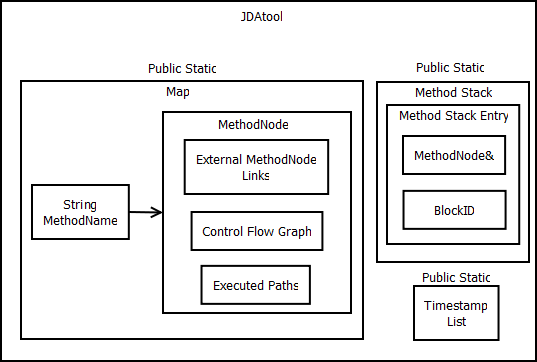
\includegraphics[width=0.48\textwidth]{JDAtool.png}
  \caption{JDA's Object Heirarchy}
  \label{fig:JDAtool}
\end{figure}

\subsection{TimestampList}
The TimestampList is essentially a list of time blocks that do not include instrumentation at the beginning and end of methods.
The small amount of instrumentation at the beginning of bytecode basic blocks, however, is too fine grain to exclude from timing.
Naturally, the instrumentation for this option occurs at the beginning end of methods.
The time that the code enters and exits instrumentation blocks can be subtracted from the overall method execution time to retrieve the native method run time.
Afterwards, blocks of times can be summed together and the extra blocks removed to save memory.
The noise, granularity, and odd JIT optimizations make the accuracy questionable for smaller methods, however large methods behave appropriately.
The featuer can be turned on by setting the trackTimes option.

\subsection{MethodNode}
The core of all method information resides in the MethodNode class.
Every unique method tag (which includes overloaded methods) reserves its own persistent MethodNode.
The MethodNodes reside in the JDAtool in a Map.
The Map allows the String typed method tags to access their respective MethodNodes.

MethodNode contains three vital pieces of information: a Control Flow Graph (CFG), a Set of ExternalLinks, and a Set of BasicBlockPaths.
The CFG contains information regarding the control flow of bytecode basic blocks in the method.
This is analyzed when the class is first loaded.
The Set of ExternalLinks contains method invocation information within that MethodNode.
They essentially keep track of the MethodNode’s basic blocks in the CFG that call other MethodNodes.
This allows us track method invocations of any sort, including invokedynamic calls.

The final data structure is the Set of BasicBlockPaths.
A method’s instrumentation can track the basic blocks that any single invocation executes.
The blocks are concatenated together to form a BasicBlockPath.
However, the BasicBlockPath implementation is somewhat unfinished; while it can recognize identical paths, it does not include loop detection.
Large or unbounded loops within a method can become very burdensome in memory with this implemetation.
As such, the option for path tracking, trackPaths, may be disabled.

\subsection{MethodStack}
The method stack is simple a list of MethodStackEntrys (MSE), where each MSE contains a MethodNode reference and an integer block ID.  
Every time a new bytecode basic block is executed, the block ID is updated.  
Every time a new method is called, that method creates a new MSE with its own MethodNode reference and adds it to the stack.  
With the MethodStack and block ID updates in each MSE, methods can extrapolate what other methods called them.  
They can then update the caller’s MethodNode with a now known ExternalLink.  
In order to track ExternalLinks, the trackBlocks option must be enabled.

\section{GUI}
The GUI is launched at the end of the main function of the instrumented program.
\section{JUNG Library}
\section{Features}

\section{Future Work}
There is a good deal of improvement that can be made to the JDA’s path tracking features.
Namely, the implementation of loop detection in paths.  
Ideally, paths should be pruned at the exit of methods by compressing loops into special subpaths.  
Loops can be simply made up of single paths or contain numerous branch statements which makes the control flow analysis hard to sort.  
There are various ways to hash loops, and thus the hashing method should be configurable.  
The concept of the JDA was more focused around tracking virtual method invocations, however the baseline instrumentation is already in place for more complex analysis.

\section{Conclusion}
We made this tool that provides information.

\bibliographystyle{./IEEE/IEEEtran}
\bibliography{report.bib}
\end{document}
